\documentclass[border=1in]{standalone}
\usepackage{tikz}
\usetikzlibrary{arrows, math}

% ensures a white background in the converted image
\pagecolor{white}

\begin{document}
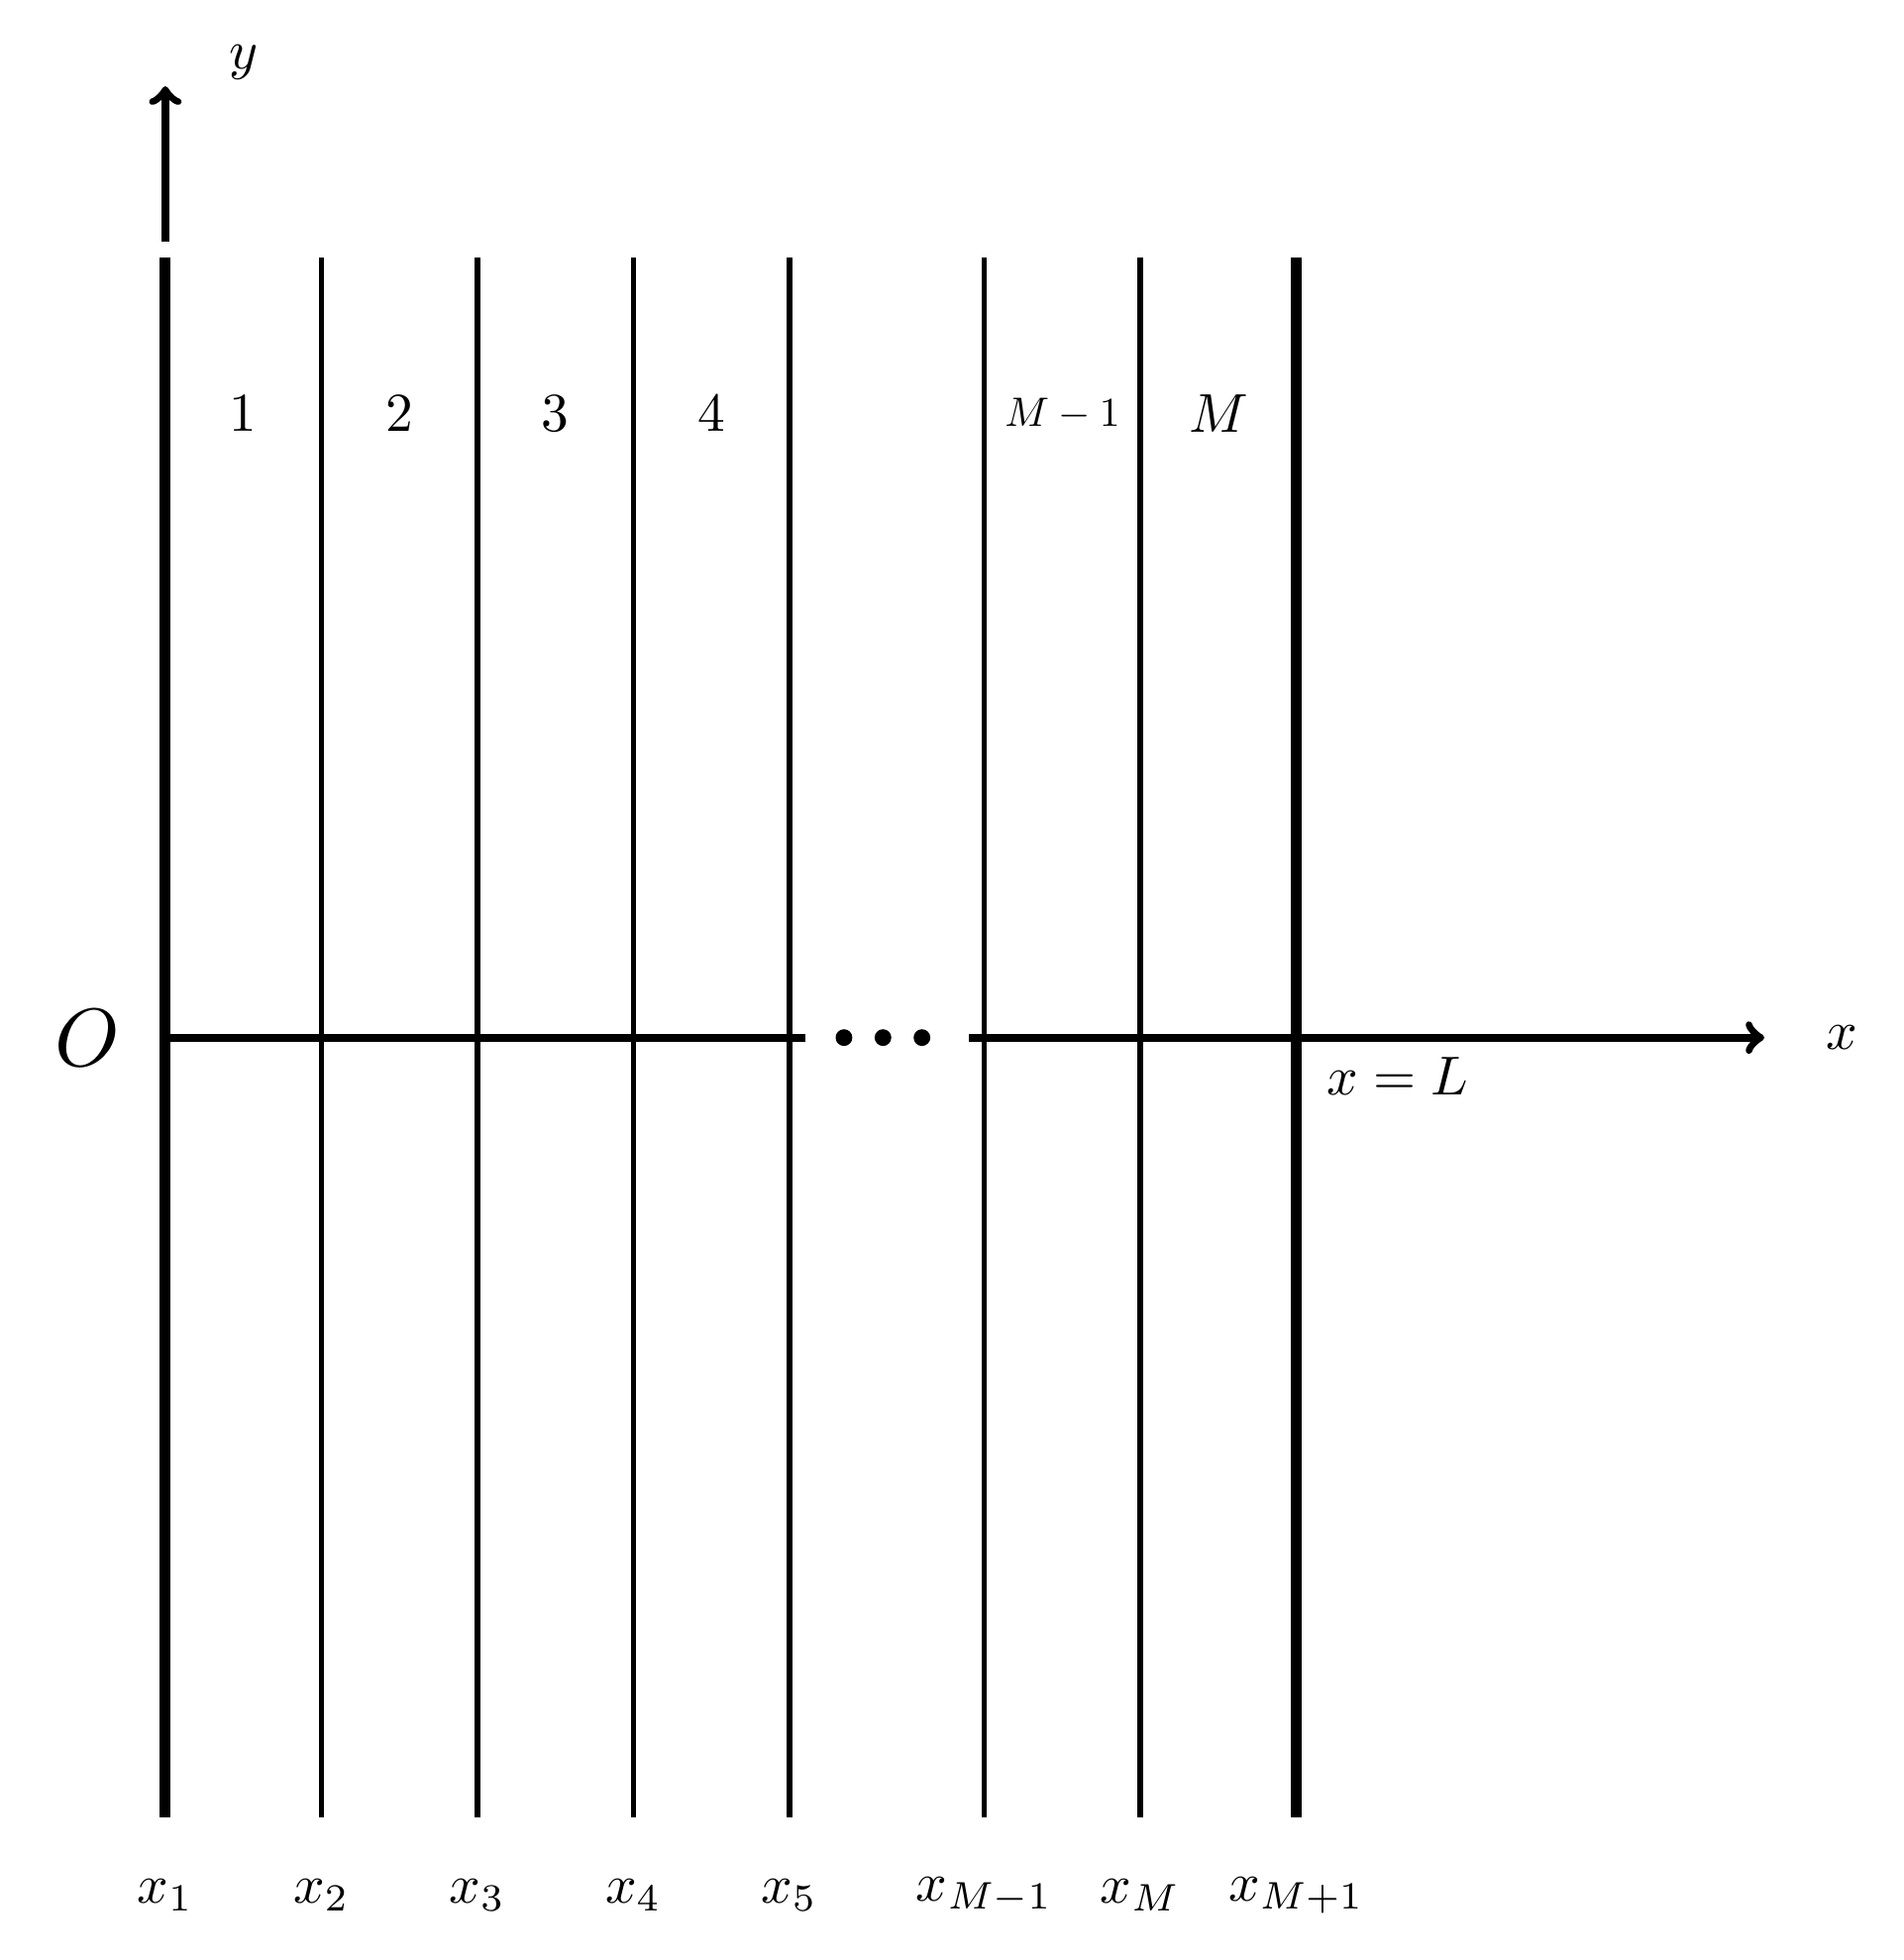
\begin{tikzpicture}
  % draw fills so lines sit on top of them
  % \fill [fill=black!60!white] (0, 0) rectangle (1, 20);
  % \fill [fill=black!20!white] (1, 0) rectangle (6, 20);
  % Draw lines
  \draw [line width=4pt] (1, 0) -- (1, 20);
  \draw [line width=2pt] (3, 0) -- (3, 20);
  \draw [line width=2pt] (5, 0) -- (5, 20);
  \draw [line width=2pt] (7, 0) -- (7, 20);
  \draw [line width=2pt] (9, 0) -- (9, 20);
  % add slightly larger gap
  \draw [line width=2pt] (11.5, 0) -- (11.5, 20);
  \draw [line width=2pt] (13.5, 0) -- (13.5, 20);
  \draw [line width=4pt] (15.5, 0) -- (15.5, 20);
  % Draw axes arrows
  \draw[arrows=->, line width=3pt] (1, 20.2) -- (1, 22.2);
  \draw[line width=3pt] (1, 10) -- (9.2, 10);
  \draw[arrows=->, line width=3pt] (11.3, 10) -- (21.5, 10);
  % Draw dots
  \draw [fill] (9.7, 10) circle (0.1);
  \draw [fill] (10.2, 10) circle (0.1);
  \draw [fill] (10.7, 10) circle (0.1);
  % Add axis and origin labels
  \node [fill=white, scale=2] at (2, 22.5) {$y$};
  \node [fill=white, scale=2] at (22.5, 10) {$x$};
  \node [fill=white, scale=3] at (0, 10) {$O$};
  % Add layer labels
  \node [scale=2] at (2, 18) {1};
  \node [scale=2] at (4, 18) {2};
  \node [scale=2] at (6, 18) {3};
  \node [scale=2] at (8, 18) {4};
  \node [scale=1.5] at (12.5, 18) {$M-1$};
  \node [scale=2] at (14.5, 18) {$M$};
  % Add interface labels
  \node [scale=2] at (1, -1) {$x_1$};
  \node [scale=2] at (3, -1) {$x_2$};
  \node [scale=2] at (5, -1) {$x_3$};
  \node [scale=2] at (7, -1) {$x_4$};
  \node [scale=2] at (9, -1) {$x_5$};
  \node [scale=2] at (11.5, -1) {$x_{M-1}$};
  \node [scale=2] at (13.5, -1) {$x_M$};
  \node [scale=2] at (15.5, -1) {$x_{M+1}$};
  % Add final position label
  \node [scale=2] at (16.8, 9.5) {$x = L$};
\end{tikzpicture}
\end{document}
